% Numbers: assets/ch4/build_progress_assets.py from the independent saved-OOF audit.
\subsubsection{Residual Diagnostics and Difficult Cases}\label{sec:residual-diagnostics}
A new calculation directly from the saved OOF predictions examines where the matched adaptation
helps and fails. These are post-hoc descriptive diagnostics on W, not new independent tests or
subgroup significance claims. Figure~\ref{fig:progress-residuals} retains every peptide, including
\nProgressBPepWorse{} that worsen with LoRA-B and \nProgressDPepWorse{} with LoRA-D.
The corresponding counts with lower MAE are \nProgressBPepBetter{} and \nProgressDPepBetter{}.
After averaging peptide differences within a protein group, B improves \nProgressBGrpBetter{}
groups and worsens \nProgressBGrpWorse{}; D improves \nProgressDGrpBetter{} and worsens
\nProgressDGrpWorse{}. Group counts describe a different weighting from peptide-macro MAE.

\begin{figure}[htbp]
  \centering
  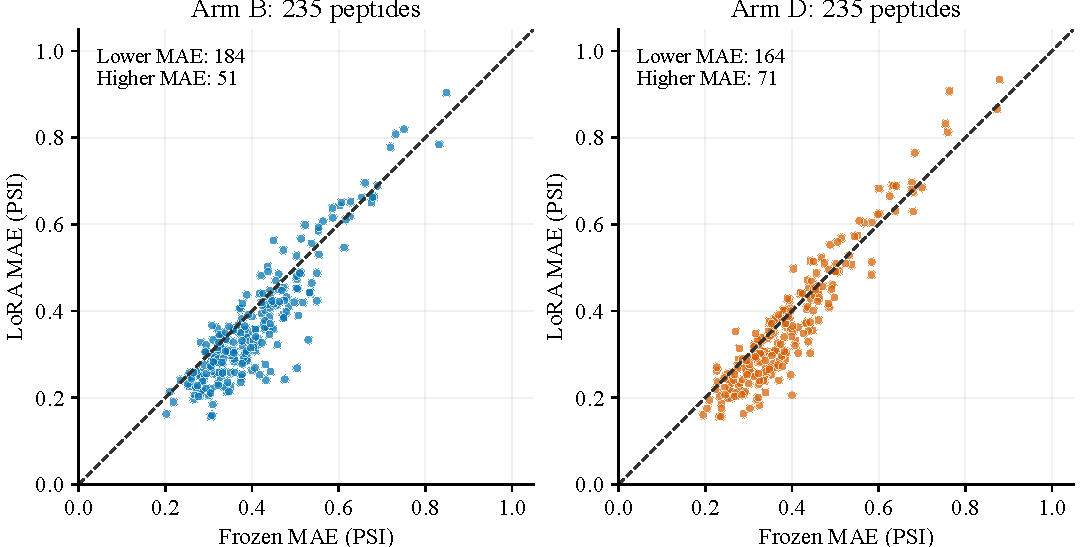
\includegraphics[width=\textwidth]{assets/ch4/fig-progress-residuals.pdf}
  \caption{Matched per-peptide OOF errors for the three-seed ensembles on W. Each point is one
  peptide; points below the dashed equality line favour LoRA. Both panels use common scales.
  The spread is observed heterogeneity, not a confidence interval.}
  \label{fig:progress-residuals}
\end{figure}

Removing each protein group in turn leaves the peptide-macro LoRA-minus-frozen MAE difference
negative: ranges are \nProgressBLeaveGroup{} for B and \nProgressDLeaveGroup{} for D.
This rules out a reversal driven by removal of any one recorded group; it does not establish
robustness to simultaneous removal of several related groups or to unobserved biological dependence.
LoRA-B fold MAEs range from 0.3384 to 0.3862 and LoRA-D from 0.3431 to 0.3882, so a global
average should not be interpreted as uniform performance. The worst LoRA-B peptide, CCDC17 tile~9,
has MAE 0.9035 versus 0.8486 for frozen-B. It remains a failure case despite the average gain.

\begin{table}[htbp]
  \centering
  \caption{OOF MAE conditional on the measured effect class ($\Delta=\Delta$PSI).
  Each metric averages errors within each eligible peptide, then over peptides in that class.
  Support counts differ from ranking eligibility, which requires at least three cells of each class.}
  \label{tab:progress-effect-errors}
  % Generated by build_progress_assets.py; descriptive OOF diagnostics.
% Source: research/progress-review-2026-11-06/local-audit.json
% SHA256: 2ea1d4235a4123bdcd0411f788f1356be6fe99b835105d1743700cf2670195a5
{\small\setlength{\tabcolsep}{3.5pt}
\begin{tabularx}{\textwidth}{Xrrrrrrr}
\toprule
Effect & Cells & Pep./grp. & Fr.-B & LoRA-B & Fr.-D & LoRA-D & Zero \\
\midrule
$-1<\Delta<1$ & 108,782 & 235/221 & 0.3270 & 0.2879 & 0.3045 & 0.2843 & 0.3031 \\
$\Delta\ge1$ & 12,053 & 198/190 & 0.8187 & 0.7997 & 0.8972 & 0.8479 & 1.4155 \\
$\Delta\le-1$ & 1,577 & 151/144 & 1.2407 & 1.0385 & 1.1394 & 0.9510 & 1.2320 \\
\bottomrule
\end{tabularx}}

\end{table}

Table~\ref{tab:progress-effect-errors} shows substantially greater errors for large effects than
for neutral cells. For $|\Delta\mathrm{PSI}|\ge1$, LoRA-B and D have MAE 0.8970 and 0.9084,
respectively, versus 1.4127 for zero, over 13,630 cells, 232 peptides and 218 groups. The positive
class has 12,053 cells; the negative class has only 1,577. LoRA-B's cell-micro signed residual
($\widehat{\Delta}-\Delta$) is $-0.9504$ for positive cells and $+1.0449$ for negative cells.
The direction is consistent with underestimating effect magnitude, but does not isolate a biological
mechanism or distinguish model shrinkage from measurement noise. These signed residuals have
different weighting from the peptide-macro absolute errors in the table.

\begin{table}[htbp]
  \centering
  \caption{Three largest absolute cell errors for LoRA-B on W, selected after inspection.
  Positions are within the measured peptide; measured and predicted values are $\Delta$PSI.
  These illustrate failures and are not clinical or mechanistic case validations.}
  \label{tab:progress-largest-errors}
  % Generated by build_progress_assets.py; descriptive OOF diagnostics.
% Source: research/progress-review-2026-11-06/local-audit.json
% SHA256: 2ea1d4235a4123bdcd0411f788f1356be6fe99b835105d1743700cf2670195a5
{\small\setlength{\tabcolsep}{4pt}
\begin{tabularx}{\textwidth}{Xrrrrr}
\toprule
Peptide & Fold & Position & Change & Measured & Predicted \\
\midrule
P32881\_IFNA8\_5 & 2 & 17 & Y$\to$F & 3.2866 & -0.1573 \\
P13942\_COL11A2\_20 & 1 & 18 & R$\to$I & 3.1698 & -0.2479 \\
P32881\_IFNA8\_5 & 2 & 17 & Y$\to$M & 3.0830 & -0.2058 \\
\bottomrule
\end{tabularx}}

\end{table}

The difficult cases in Table~\ref{tab:progress-largest-errors} include sign reversals for strongly
stabilising measured substitutions. Post-hoc tables by mutant amino acid and by WT--replacement
pair are retained in the accompanying audit with support counts. Their uneven support and shared
protein contexts prevent interpreting a high subgroup error as a causal residue-specific mechanism.
